\documentclass[e4_tp2_main.tex]{subfiles}
\begin{document}
\newgeometry{top=2.5cm, bottom=2.0cm, left=2.25cm, right=2.25cm}

\section{Convertidor Boost para Lámpara LED de potencia}

\subsection*{LED's de Potencia: Efecto de la temperatura - Realimentación}
De la hoja de datos de OSRAM para el LUW-W5AP, se da la curva de $\Delta V(T)=V_F-V_F(25^{\circ})$, para la corriente $I_F$ máxima de 1400mA. La misma tiene pendiente negativa, es decir, que a mayor temperatura, la tensión en directa sobre el LED disminuye.

\begin{figure}[H]
\centering
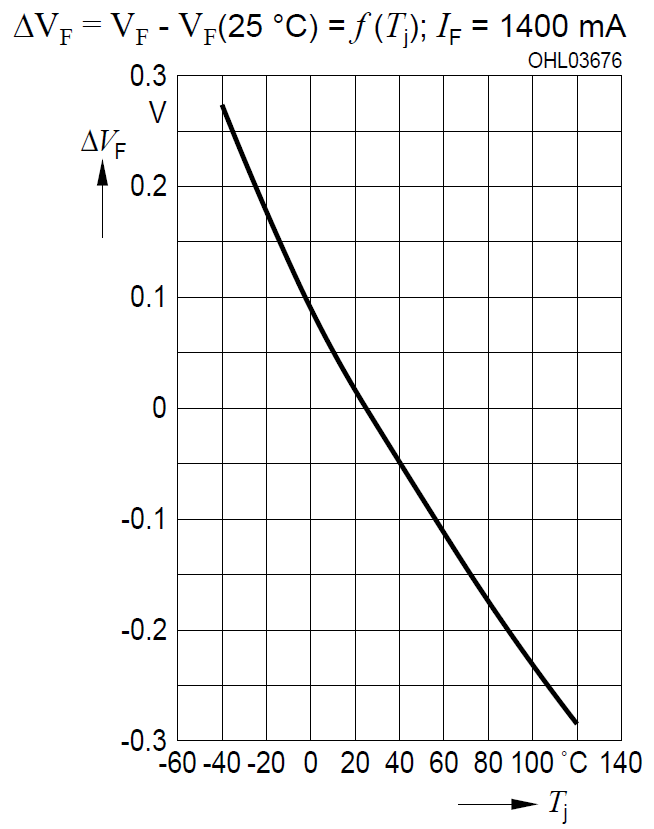
\includegraphics[width=0.3\linewidth]{Imagenes/Punto2/efectoT.png}
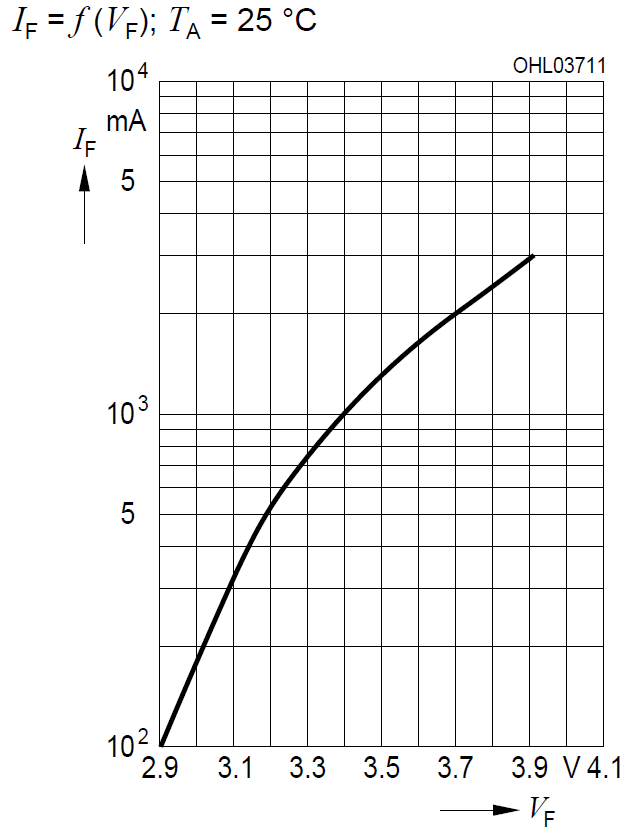
\includegraphics[width=0.29\linewidth]{Imagenes/Punto2/IF-VF.png}
\caption{Efecto de la temperatura en la $V_{LED}$: $\Delta V_F(T_j)$ - Curva de $I_F(V_F)$}
\end{figure}

Al trabajar con LED's de potencia, es conveniente realimentar la corriente en lugar de la tensión. Esto se debe a que si se produce una perturbación en la carga (es decir, para el caso de la simulación cortocircuitar dos LED's), si se está regulando tensión, caerá más tensión sobre los LED's restantes, por lo que la corriente aumentará, de acuerdo a la curva de $I_F(V_F)$ provista en la hoja de datos. Esto podría llevar a que los LED's se quemen por exceso de potencia.

\subsection*{LED's de Potencia: Variación del Brillo}
En el realimentador, el amplificador operacional amplifica la tensión sobre la resistencia sensora de la corriente ($R_2$), de manera de obtener a su salida la tensión de referencia de 2.5V para el LT1241. El lazo de realimentación ajusta la corriente para tener en el Pin 2 (FB) dicho valor de tensión dado que el operacional interno a la entrada se encuentra realimentado negativamente de forma externa con un RC entre su salida y el Pin 2 (que es la entrada inversora). Internamente, la entrada no inversora está a un potencial constante de 2.5V. Como el operacional realimentado negativamente busca llegar a que $V^+ = V^-$, de ahí obtenemos que la entrada del Pin 2 se lleva a 2.5V.\par
Teniendo esto en cuenta, Se busca en la hoja de datos el valor de corriente para el cual se obtiene la mitad del brillo (para el valor actual de 2A se obtiene el máximo). De acuerdo a la curva provista:

\begin{figure}[H]
\centering
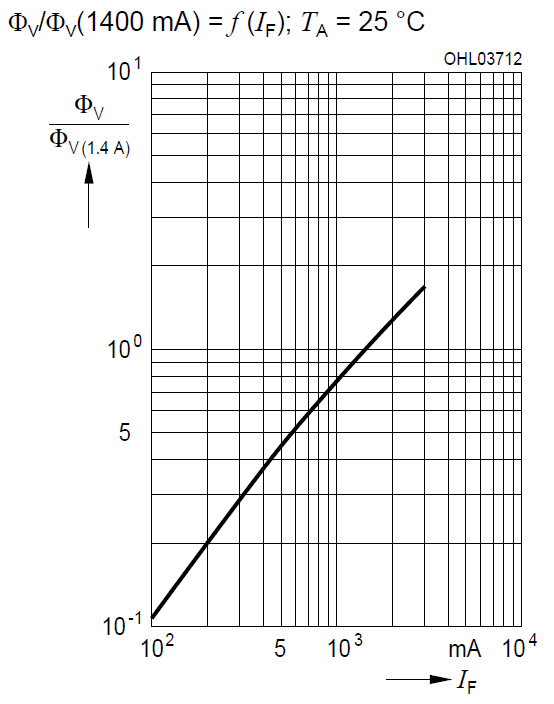
\includegraphics[width=0.3\linewidth]{Imagenes/Punto2/Lumen-IF.png}
\caption{Curva de $\frac{\Phi_V}{\Phi_V(1.4A)}(I_F)$}
\end{figure}

Se tiene que la mitad del brillo máximo se da a una corriente 
de 700mA. Por lo tanto, la tensión sobre la resistencia sensora $R_2$ será de: 

\[
I_F = 700mA \cdot 0.1\Omega = 0.07V
\]

Sabiendo que a la salida del operacional debe haber 2.5V, se despeja el nuevo valor para $R_6$:
\[
\frac{2.5V}{0.07V} = G = 35.7 \longrightarrow R_6 = 34.7K \Omega
\]

\subsection*{Oscilador - Frecuencia de Switching}
De la hoja de datos, en la sección de Oscilador, se indica que la frecuencia del LT1241 es el doble que la de switching. Entonces, para tener 75KHz, se buscará en la gráfica de $R_TC_T(f)$ el par de valores de componentes acordes para una frecuencia de 150KHz:

\begin{figure}[H]
\centering
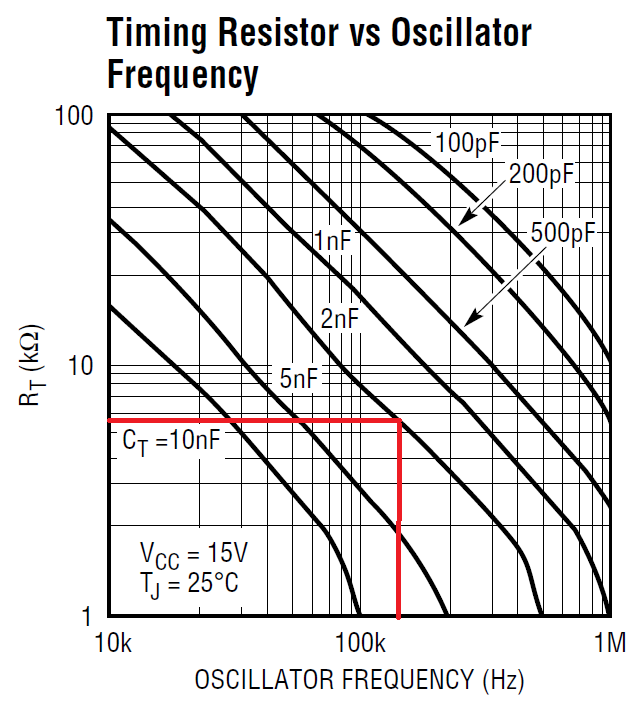
\includegraphics[width=0.3\linewidth]{Imagenes/Punto2/RT-OSC.png}
\caption{Curva de $R_TC_T(f)$}
\end{figure}

De donde se obtiene $R_T = 5.3K\Omega$ y $C_T = 2nF$. Es posible verificar mediante las ecuaciones provistas en la misma hoja:

\[
t_r = 0.583 \cdot R_T \cdot C_T \hspace{2cm} t_d = \frac{3.46 \cdot R_T \cdot C_T}{0.0164 \cdot R - 11.73}
\]
\[
T_{OSC} = t_r + t_d \longrightarrow f_{OSC} = 150KHz
\]
\[
f_{SW} = \frac{f_{OSC}}{2} = 75KHz
\]

\subsection*{Perturbaciones sobre el circuito}
Se analizarán dos casos: aplicando un escalón de carga (cortocircuitando 2 LED's), y aplicando un escalón de alimentación (pasando la fuente de entrada de 12V a 15V).
\subsubsection*{Perturbaciones en la carga}
\begin{figure}[H]
\centering
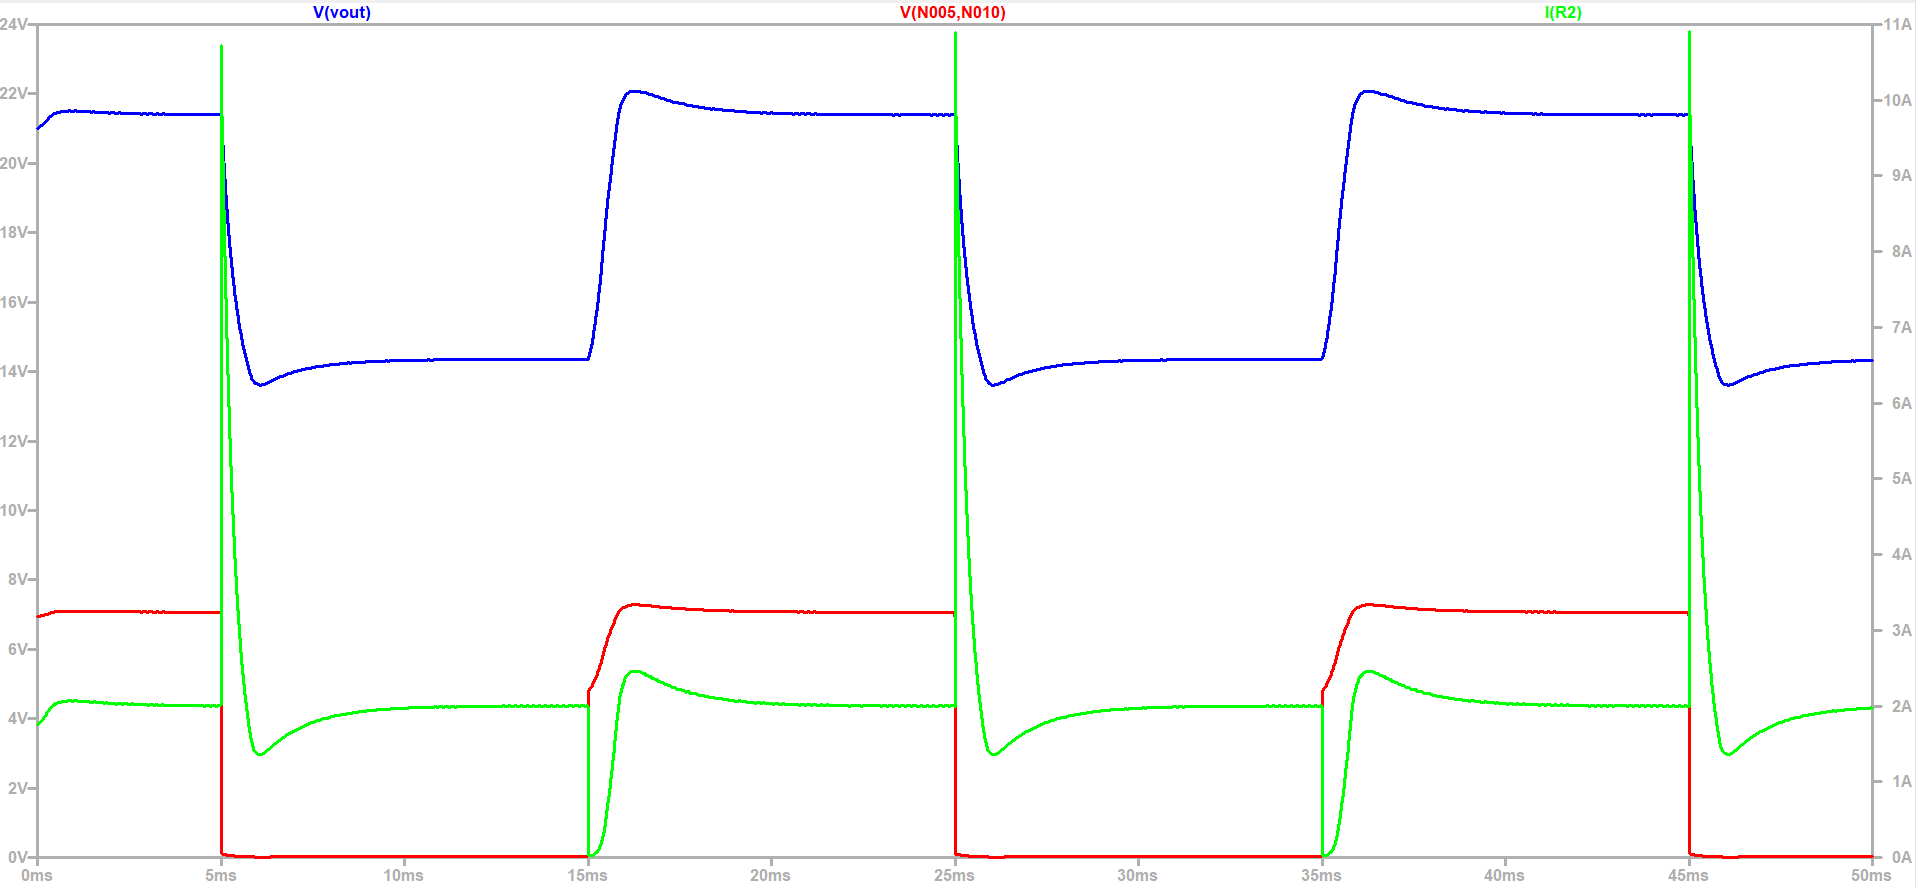
\includegraphics[width=0.7\linewidth]{Imagenes/Punto2/cargavariable-I-V.png}
\caption{Respuesta frente a escalón de carga: $I_o$ (Azul) - $V_{n007}$ es el SW (Rojo) - $V_o$ (Verde)}
\end{figure}

Al producir el escalón de carga (cuando la tensión en el Sw pasa a 0V), como se tiene la misma tensión en dicho instante para una menor cantidad de LED's ahora, se observa entonces un pico de corriente positivo. Esto es debido a que el aumento de tensión en los LED's se traduce en un aumento exponencial de la corriente, debido a la relación $V_D(I_D)$. A medida que el lazo de realimentación vuelve a llevar la corriente hacia el valor regulado de 2A, la tensión en los LED's restantes disminuye, por lo que la tensión de salida disminuye. Cuando se vuelven a agregar los 2 LED's, ocurre lo opuesto, es decir, un pico negativo de corriente (casi hasta 0A), dado que la misma tensión sobre más LED's ahora se distribuye, porque dada la relación $V_D(I_D)$ es de esperar que la corriente disminuya. Luego el lazo la lleva al valor regulado de 2A, aumentando en consecuencia la tensión.

\subsubsection*{Perturbaciones en la fuente}
\begin{figure}[H]
\centering
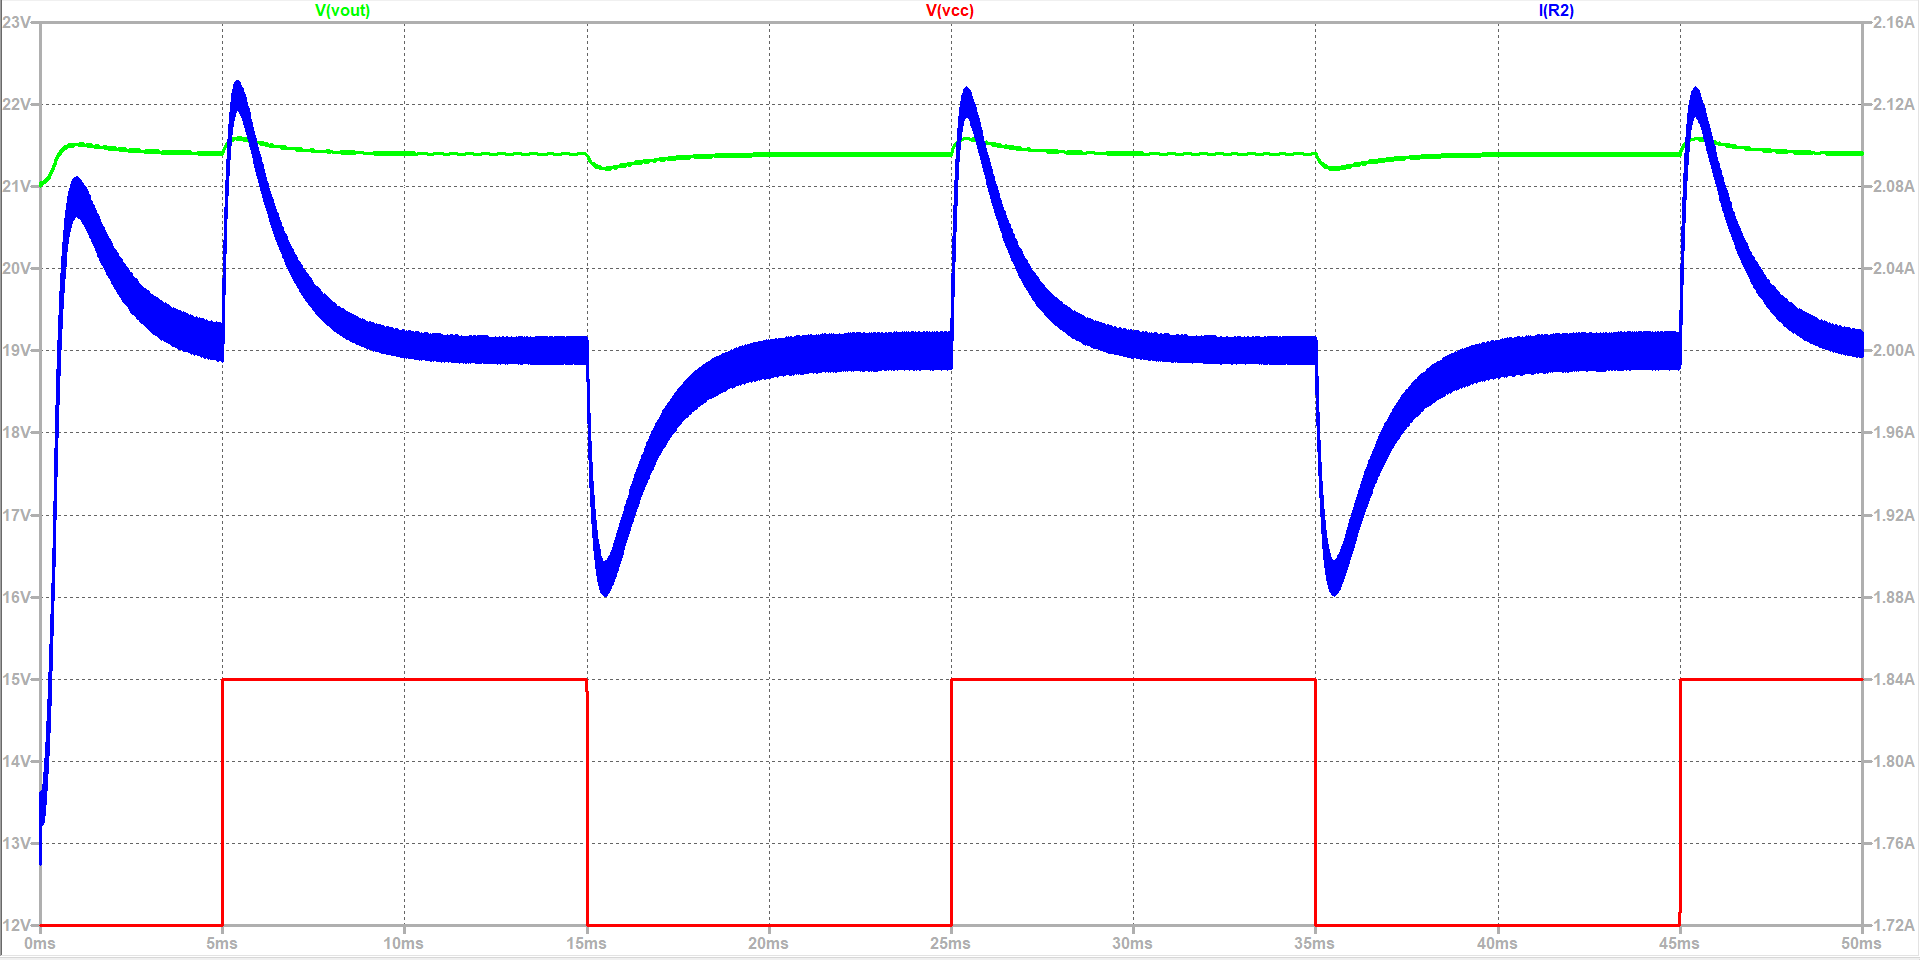
\includegraphics[width=0.7\linewidth]{Imagenes/Punto2/fuentevariable-I-V.PNG}
\caption{Respuesta frente a escalón de tensión: $I_o$ (Azul) - $V_{vcc}$ es la entrada (Rojo) - $V_o$ (Verde)}
\end{figure}

En la imagen se muestra que, frente al escalón en la tensión de entrada, un aumento tanto en la tensión de salida como en la corriente (este último con mayor zoom). Para ambos, el porcentaje de aumento es mucho menor que en el caso de escalón de carga, en particular el de la corriente es solamente de un 5\% de su valor nominal. Como la tensión de salida se mantiene casi estable frente a perturbaciones en la entrada, es de esperar que la corriente, por consiguiente, no varíe en mayor proporción.

\newpage

\subsection*{$\mathbf{I_{PK}(I_O)}$ - Corriente pico en el switch en función de $\mathbf{I_O}$}


Teniendo en cuenta que en un circuito Boost se sabe que la corriente máxima del switch coincide con la corriente máxima en la bobina por ende se puede decir que:
\begin{equation}
I_{L(max)}=I{pk}=\frac{I_{out}}{1-D}+\frac{V_{in}*D}{2*L*f_s}
\end{equation}
Cuyo duty cycle(D) viene dado por:
\begin{equation}
D=1-\frac{V_{in}}{R_L*I_{out}}
\end{equation} 

En donde $R_L$ representa la carga total del circuito que la podemos representar como $R_L=R_{LED}+R_2$ donde $R_2$ es la resistencia utilizada para medir corriente. Dicho esto y reemplazando en las ecuaciones anteriores se llega a la siguiente expresión:
\begin{equation}
I_{L(max)}=I_{pk}=\frac{I_{out}^2*R_L}{V_{in}}+\frac{V_{in}*\left(\frac{V_{in}}{I_{out}*R_l}\right)}{f_s*2*L}
\end{equation}
El valor que puede tomar $I_{out}$ está limitado por el diodo zener que posee el integrado LT1241 utilizado, el cual funciona como clamper de 1V si se excede dicho valor. Segun la datasheet dicha corriente es $I_{pk}=\frac{V}{R4} $ donde  $ 0 \leq V \leq 1V$ lo que establece una corriente máxima de $I_{pk}=\frac{1V}{R4}$. Por lo tanto el valor que tomará la corriente en el switch está determinado de la siguiente manera:
\[
I_{pk}= \left\{ \begin{array}{lcc}
             \frac{I_{out}^2*R_L}{V_{in}}+\frac{V_{in}*\left(\frac{V_{in}}{I_{out}*R_l}\right)}{f_s*L} &   \textrm{si}  & I_{min}\leq I_{out} \leq I_{max}  \\
             \\ \frac{1V}{R4} &  \textrm{caso contrario} \\
             \end{array}
   \right.
\]   
Donde el valor máximo y mínimo se obtienen al reemplazar por los valores de dichos componentes. Cuando se limita la corriente se dice que este circuito entra a trabajar en condiciones de falla ('Fault Conditions' según el fabricante), ya sea por un cortocircuito o por un escalón de carga.


\subsection*{Función de Blanking}

El problema al que responde esta función es sobre el ruido producido en la entrada $I_{Sense}$, debido a los picos de corriente que ocurren en la conmutación del transistor, como la $I_{rr}$ del diodo. Puede provocar una desviación excesiva en el duty del PWM.\par
La función de blanking (ubicada a la salida del comparador de $I_{Sense}$) lo que hace es retener la salida de dicho comparador cuando el transistor conmuta, durante un breve período de tiempo fijo. De esta forma se previene el inconveniente anterior sobre el PWM. Esta función evita tener que agregar un filtro en la entrada $I_{Sense}$, que provocaría un mayor tiempo de respuesta en la realimentación de corriente.\par
El tiempo de blanking es función de la tensión en el pin de feedback (Pin 2). Para condiciones normales de operación ($V_{FB} = 2.5V$), el tiempo es de 100nS, y disminuye a cero si se lleva a cero dicha tensión. Esto quiere decir que el tiempo de blanking es mínimo cuando se enciende el circuito y durante un cortocircuito en la salida. 

\newpage

\subsection*{Eficiencia de la Fuente}
Para obtener el rendimiento de la fuente, se calcula la potencia entregada por la fuente y la potencia de salida:

\[
P_i = V_d \cdot I_d = 12V \cdot 4A = 48W  
\]
\[
P_o = V_o \cdot I_o = 21.4V \cdot 2A = 42.8W
\]

Por lo que el rendimiento de la fuente en relación entrada/salida es:
\[
\eta \% = 100 \cdot \frac{P_o}{P_i} = 89.2 \%
\]
Por lo que el resto de las potencia son las pérdidas en los elementos, a calcular a continuación.\par

Las pérdidas en el transistor se calculan midiendo los tiempos de conmutación, mediante la ecuación:

\[
P_d = \frac{1}{2} \cdot V_{ds} \cdot I_d \cdot (t_{ri} + t_{fv} + t_{fi} + t_{rv}) \cdot f_{sw} = 1.1W
\]

Para las pérdidas en el diodo, se calcula con el valor medio, es decir mientras conduce (no se tiene el cuenta las pérdidas por $I_{rr}$ dado que no es representativa en comparación a las pérdidas durante todo el tiempo de conducción del diodo):

\[
P_D = I_D \cdot V_D \cdot t_{off} \cdot f_{sw} = 2W
\]

Para las pérdidas en las resistencias de sensado de $I_{sw}$ y de $I_o$:

\[
P_{R} = I_{sw} \cdot V_{R4} \cdot t_{on} \cdot f_{sw} + I_o \cdot V_{R2} = 1.2W  
\]

Las pérdidas en el controlador PWM, ocurren mayormente durante el encendido del transistor. Midiendo el tiempo que dura dicha corriente, se tiene:

\[
P_{IC} = I_c \cdot V_{cc} \cdot t_{on-Isw} \cdot f_{sw} = 0.08W
\]

\begin{table}[h]
\centering
\begin{tabular}{|l|c|c|}
\hline
Componente                        & \multicolumn{1}{l|}{Pérdida de potencia} & \multicolumn{1}{l|}{\% Sobre el total} \\ \hline
Transistor MOSFET                 & 1.1W                                     & 2.3\%                                  \\ \hline
Diodo de potencia                 & 2W                                       & 4.2\%                                  \\ \hline
Controlador PWM                   & 0.08W                                    & 0.2\%                                  \\ \hline
Resistencias para medir corriente & 1.2W                                       & 2.1\%                                  \\ \hline
\end{tabular}
\end{table}

Donde se observa que las mayores pérdidas se dan sobre el diodo en tiempo de conducción.

\end{document}